\documentclass[12pt]{article}
%Required: You must have these
\usepackage{graphicx}
\usepackage{tabularx}
\usepackage{natbib}
\usepackage{lineno}
\linenumbers

\usepackage{array}
\usepackage{amsmath}
%\usepackage[backend=bibtex]{biblatex}
\setkeys{Gin}{width=0.8\textwidth}
%\setlength{\captionmargin}{30pt}
\setlength{\abovecaptionskip}{10pt}
\setlength{\belowcaptionskip}{10pt}
 \topmargin -1.5cm 
 \oddsidemargin -0.04cm 
 \evensidemargin -0.04cm 
 \textwidth 16.59cm
 \textheight 21.94cm 
 \parskip 7.2pt 
\renewcommand{\baselinestretch}{1.2} 	
\parindent 0pt

\bibliographystyle{..//..//refs/bibstyles/amnat.bst}
\usepackage{xr-hyper}
\usepackage{hyperref}


\title{
Patterns of spring-freeze risk across the geographic ranges of temperature trees contributes to their phenological cue differences, but leaves much unexplained\\
Other
}

\author{Dan, Cat, Nacho, Ben Cook, Faith, Deidre, Mira Geoff and Lizzie}
\usepackage{Sweave}
\begin{document}
\Sconcordance{concordance:rangeredo.tex:rangeredo.Rnw:%
1 35 1 1 0 64 1}

\maketitle

\section*{Abstract}
\section*{Introduction}


Phenology, the timing of annual life cycle events, allows for organisms to match critical life-cycle transitions with optimum environmental conditions. Through the phenology of spring budburst, temperate woody balance the advantages of precocious growth resumption for resource gains with the risk of damage from late season freezes \citep{Savage:2013aa}. To navigate this trade-off, woody plants have evolved complex physiological responses to sense environmental cues that signal the arrival of appropriate conditions for resuming growth \citep{}.Decades of research on phenology have elucidated these environmental cues, suggesting that warming spring temperatures (forcing), cool winter temperatures (chilling) and day length (photoperiod) are primary environmental cues utilized by woody plants to determine the timing of spring phenological events \citep{Ettinger:2020aa,Forrest2010}. Yet These studies also demonstrate the there are substantial cue-use differences among species, with some species relying more heavily on some cues over others \citep{Laube:2014aa}. However, our knowledge about why species differ in their cue responses is currently limited, and nderstanding the ecological and evolutionary drivers that shape phenological cues is critical for our ability to the magnitude and impacts of phenological shifts with climate change.


The predictability of the arrival spring may strongly influence the evolution of phenological cues \citep{Zohner:2017aa} (Zohner2 and Dawson Glass). In regions where the start of spring is unpredictable, species should evolve stronger dependence on chilling and photoperiod cues to prevent premature leafout and exposure to frost damage. In contrast, in regions where the seasonal warming reliable indicate the start of spring, species should depend respond strongly to forcing and not chilling or photoperiod. This spring predictability hypothesis (hereafter:SPH) is both intuitive and has found some recent support in the literature \citep{Zohner:2017aa}. However, the SPH hinges on the assumption that species phenological responses are at a stable equilibrium with their environment, as assertion that is highly contested \citep{}. It is also unclear the time scale at which season predictability shapes cue responses. Spring predictability could drive selective pressure to the increase chilling and/or photoperiod sensitivity on an evolutionary time scale, or define species ranges based on their inhereted cue sensitivies on an ecological time scale. Testing the predictions of SPH across multiple geographic scales can serve to evaluate this hypothesis, and offer an improved understanding of the drivers of biogeographic patterns of phenology cue sensitivity.

\section*{Continental Climatic Pattern}

Global circulation patterns generate substantially different spring climatic conditions on either side of the North Atlantic \citep{}. In Eastern North America, the spring is marked by instability, while in Europe, the arrival of spring is consistent and nice (Figure 1). Given these contrasting climate regimes, the SPH predicts that North American species should have stronger sensitivity to chilling and photoperiod and weaker to forcing \citep{Dawson Glass}. We tested these predictions using phenological observations from the OSPREE database  with Bayesian Hierarchical models developed by \citet{Nacho} to estimate species level cues and account for phylogeny. We compared the cue sensitivites of North American and Europe species by extracted all species level posterior estimates for forcing, chilling and photoperiod sensitivity and grouping them  by continent to which species' were native (See Supporting Information: Methods for details).

There were no substantial differences in clue sensitivity between continents (Fig 2). Mean forcing sensitivity for European species was X  and Y for North American species. Mean chilling sensitivity for European species was X  and Y for North American species. Mean photoperiod sensitivity for European species was X  and Y for North American species.

While finding does not lend support to the SPH, it is not particularly surprising given that recent studies have found thre to be strong phylogenetic conservatism in phenological cue responses, and that there are many closely related congeners found in both North America and Europe. It is therefore likely that patterns of cue use diverged among taxa well before the modern placement of continents, under different climate conditions than North America and Europe experience today. (wow say better).  

This finding calls into question the recent assertion that European plant species successfully invade North American ecosystem because their higher reliance on forcing cues allows them to leafout earlier and gain a growth advantage over their competitors (Dawson Glass). While these kinds phenological priority effects have been documented as contributing to the success of invaders (Buonaiuto, others) our findings indicate that other mechanisms are likely more important for explaining the success of European woody plants in North America. Instead, this finding may help us understand why many European timber species have been successfully established in Northern America (and visa versa), without becoming aggressive on the landscape.

\section*{Range Patterns}
Instead of continental-scale patterns of biogeography driving divergent evolutionary trajectories of cue use, it is also possible that phenological responses to cues play a more important role in determining species range limits (Chuine). The distributions of species that rely primarily on forcing, should be restricted geographic regions where spring predictability is high, while species that rely more heavily on chilling and photoperiod can persist in regions where spring predictability is low. If this is the case, the SPH predicts that within each continent, species with higher chilling and photoperiod cue responses should be associated with lower spring predictability across their ranges.

We tested this prediction by regressing the species-level posterior estimates of forcing, chilling and photoperiod sensitivity from our previously described model against the two metrics of spring predictability: the standard deviation in growing degree days to last frost and Spring Temperature Variability (STV) defined as the standard deviation of mean minimum temperature from March-May \citep[See Supporting Information Methods]{Zohner:2017aa}. We analyzed this relationship between spring predictability and cue responses using a Bayesian hierarchical framework, with separate models for each cue by continent (see Supporting Information: Methods for details). 

In Europe, differences in spring predictability across species ranges didn't related to chilling or photoperiod cue sensitivity. In contrast, in North America lower spring predictability was related to higher chilling sensitivity and lower forcing sensitivity as predicted by the SPH. 

This pattern qualitative matches previous tests of the SPH that found stronger relationships between spring predictability and phenological cue sensitivity in North America than in Europe \citep{Zohner:2017aa}. Our findings are even more stark---we only found evidence for the SPH in North America. We can understand this pattern by comparing the variation in spring predictability across species ranges in each continent. In Europe, not only is spring predictability generally high, it is relatively stable across the whole continent. In contrast, there is much more variation across North America (Figure 1). In Europe, the magnitude of climate variation is simply insufficient to impose sort species ranges based on their cue responses. But in North America it is.

\section*{Does local adaptation swamp the SPH}
One possible reason for the weak support for the SPH we found in our analyses is that local adaptation in phenological cue sensitivity overwhelms any relationship between species-level cue use and range-wide climate conditions. If cues are locally adapted, it follows that neither continental differences or range wide climate conditions would be strongly associated with cue use. 

To assess this possibility in our data, we designed a two-level, hierarchical model for studies in the OSPREE database that sampled species from multiple provenance locations.We model study, species and population as intercepts, forcing and photoperiod as predictors (fixed effects) with species nested within population (i.e., site) as modeled groups (random effects). While we detected limited population level variation in forcing and photoperiod cue sensitivity, though this within species variation was less substantial than among species variation (Fig. \ref{fig:popy}). Notably, we found the largest source of variation in phenological cue estimates was the study effect Fig. \ref{fig:popy}). This result does not support the assertion that local adaptation is masking relationships between cue sensitivity and range-level climatic patterns.

\section*{Phenological cue differences: More than climate drivers}

Our results do not support the simple predictions of the Spring Predictability Hypothesis. This lack of support does not inherently challenge the theoretical importance of spring predictability in driving selection of cue sensitivity, but calls into question the wisdom of related differences in phenological sensitivity to the contemporary environmental conditions that species experience in their present ranges. As mentioned above, several studies have identified a strong a phylogenetic signal in cue sensitivity (Nacho and Others), suggesting that if spring predictability shaped modern-day cue responses in woody plants, we would need to look to the paleo-environment to see such as association. The lack of support for the SPH further support evidence that species phenological responses are not in equilibrium with their environment---we know that species ranges are still rebounding from the most recent glacial period (). In North America, where the predictability of spring varies substantially across the the continent, high chilling sensitivity may have allowed some species to expand their ranges into regions where spring predictability is low but this patterns was not apparent in Europe, where spring predictability is consistently high across the continent.

While the combination of strong phylogenetic conservation and climate disequilibrium is alone a good enough explanation for why this relationship is weak, there are other selective factors may be drivers of cue differences among species. Recently studies have connected phenological cues to functional traits (Deirdre) community assembly, and niche partitioning (). The role of community interactions in shapping cue sensitivity patterns within a community could be explored more (Maybe Lizzie has more to say on this based on her coexistence review).

\section{Conclusion:}
In this study we found limited support for the assertion that the predictability of spring that species encounter across their geographic ranges shape their relative reliance on forcing, chilling and photoperiod cues for spring phenology. Our results suggest that climate variability may drive cue use pattern only when it is sufficiently high, like in contemporary North America. These results suggests that future studies of phenological cue-use would benefit from a holistic integration of these bio-climatic hypotheses with phylogenetic, functional trait, and climatic legacy hypotheses to fully understand the evolution of phenological cues in woody plants, and how cue use patterns will impact species performance in the face of global change at across multiple spatial and temporal scales.

\bibliography{..//..//refs/ranges}
\section*{Figures}

\begin{figure}[h!]
    \centering
 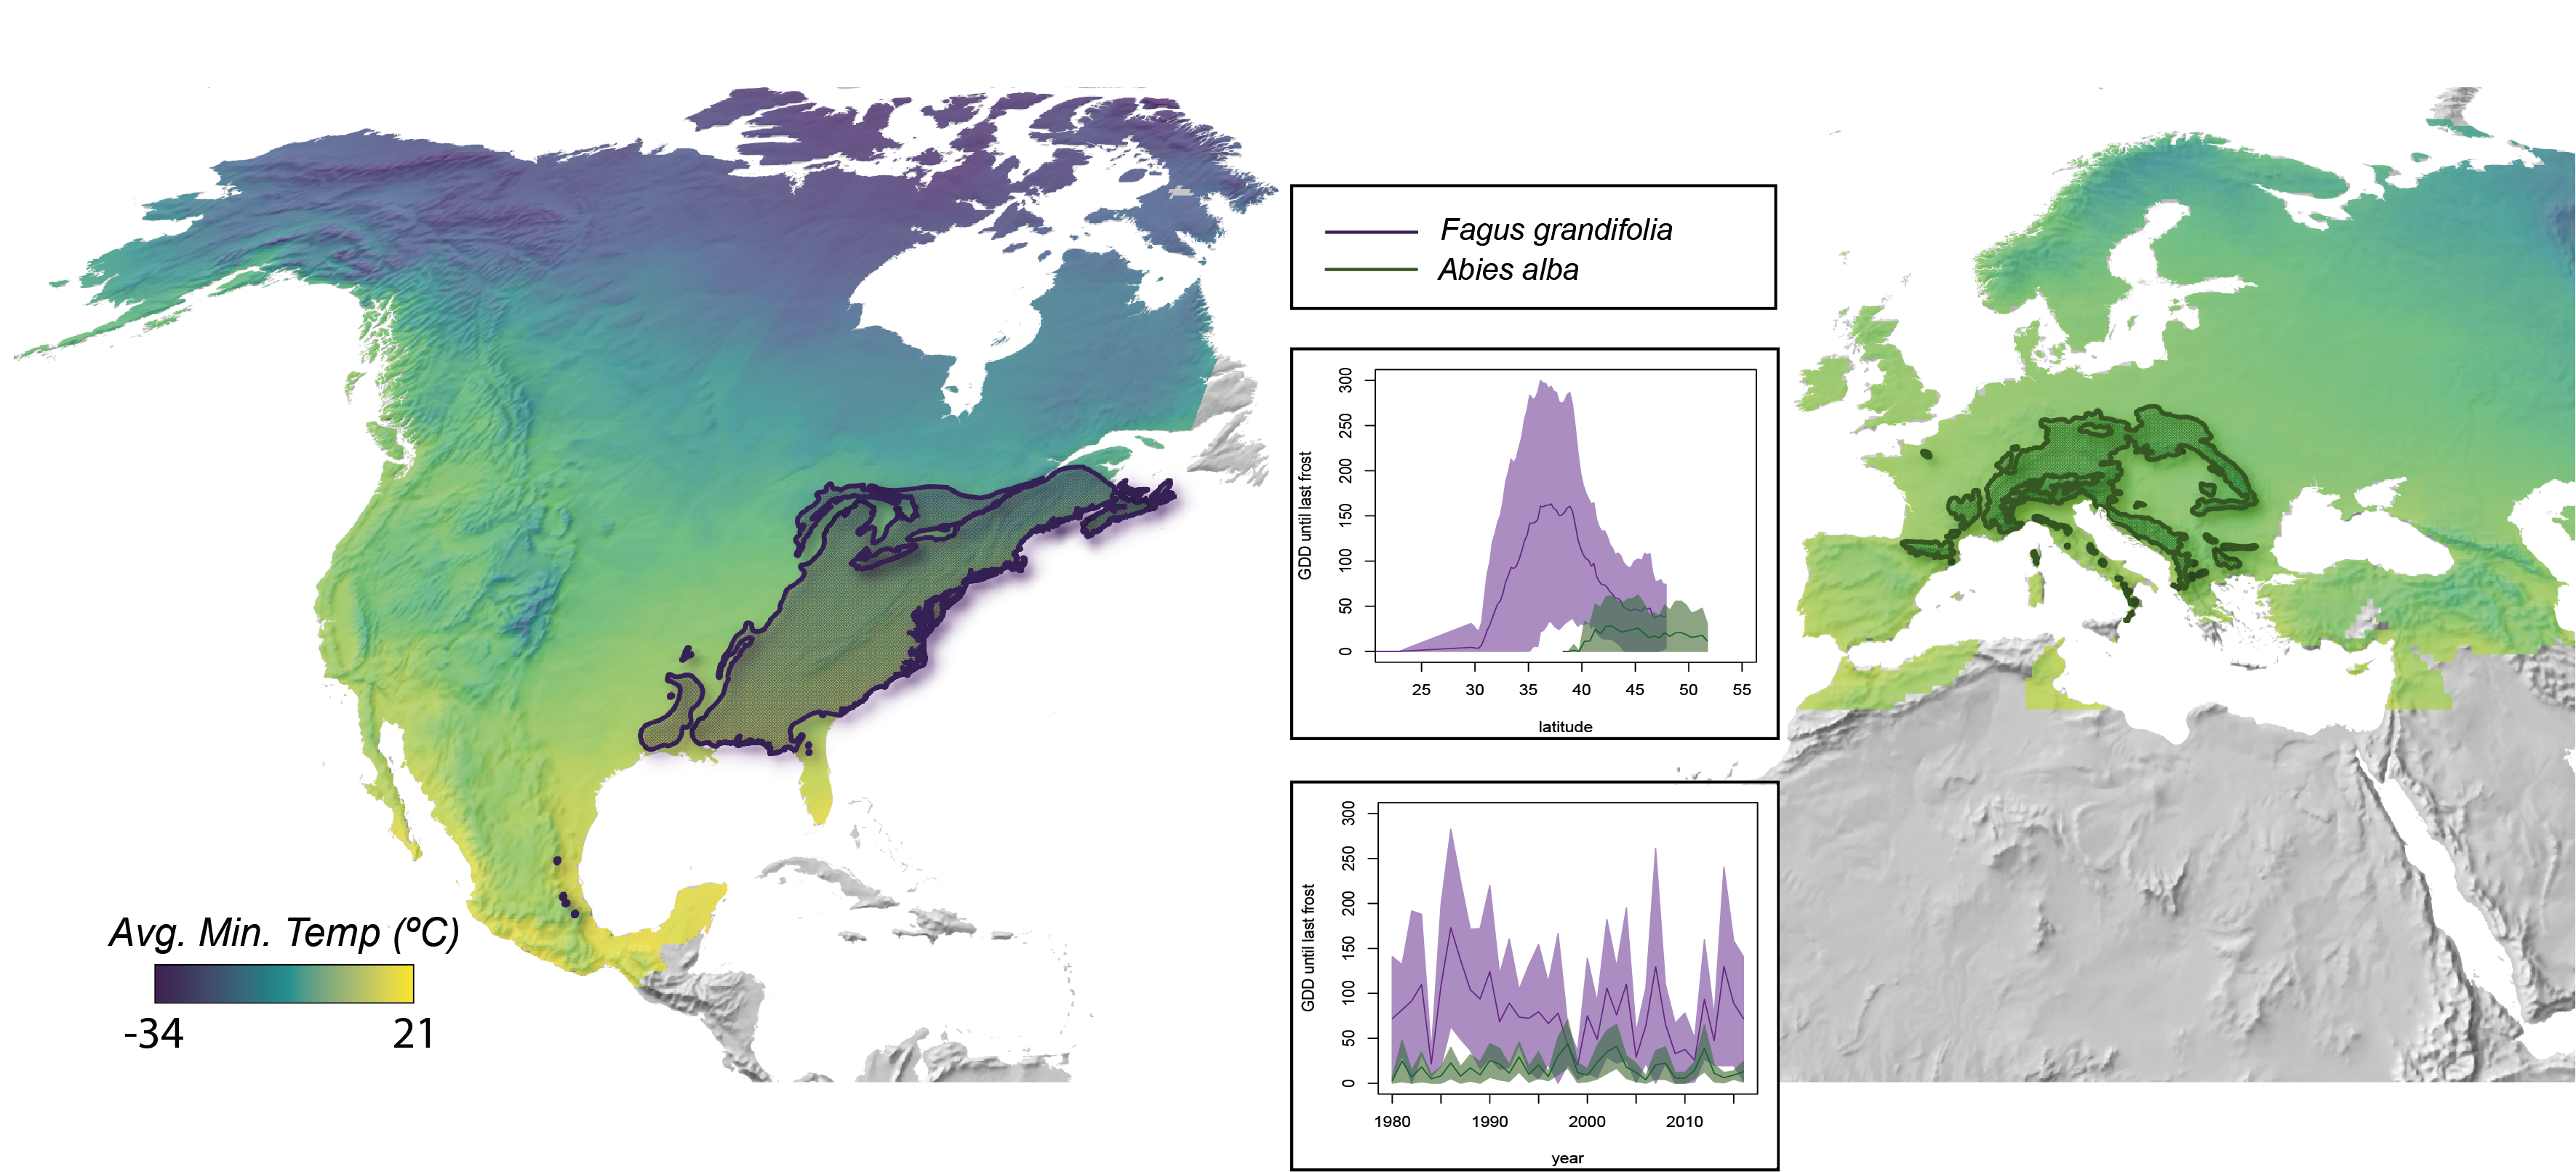
\includegraphics[width=\textwidth]{..//..//analyses/ranges/figures/concept figure draft2.png} 
    \caption{I am now thinking we should just have a figure comparing Spring variability on North America vs. Europe}%Illustration of the marked continental differences in spatial and temporal variation of climate within the geographic range of two example species: \emph{Fagus grandiflora} in purple and \emph{Abies alba} in green. The map shows the contrast between minimum temperatures averaged during winter across continents and how overlaid species' ranges may encompass different amount of variation in these temperatures. The insets show latitudinal (upper) and temporal (bottom) variation in Growing Degree Days recorded until the last day of frost (GDDlf) within each species range. It is to note that even if the European species' range reaches higher latitudes than the North American species, its climatic variation is sensibly smaller both temporally and spatially.}
    %Nacho, do you want to try taking a stab at this caption? I am happy to work on it if you want to start by just jotting a few notes/ideas down
    \label{fig:concept}
\end{figure}

\begin{figure}[h!]
    \centering
 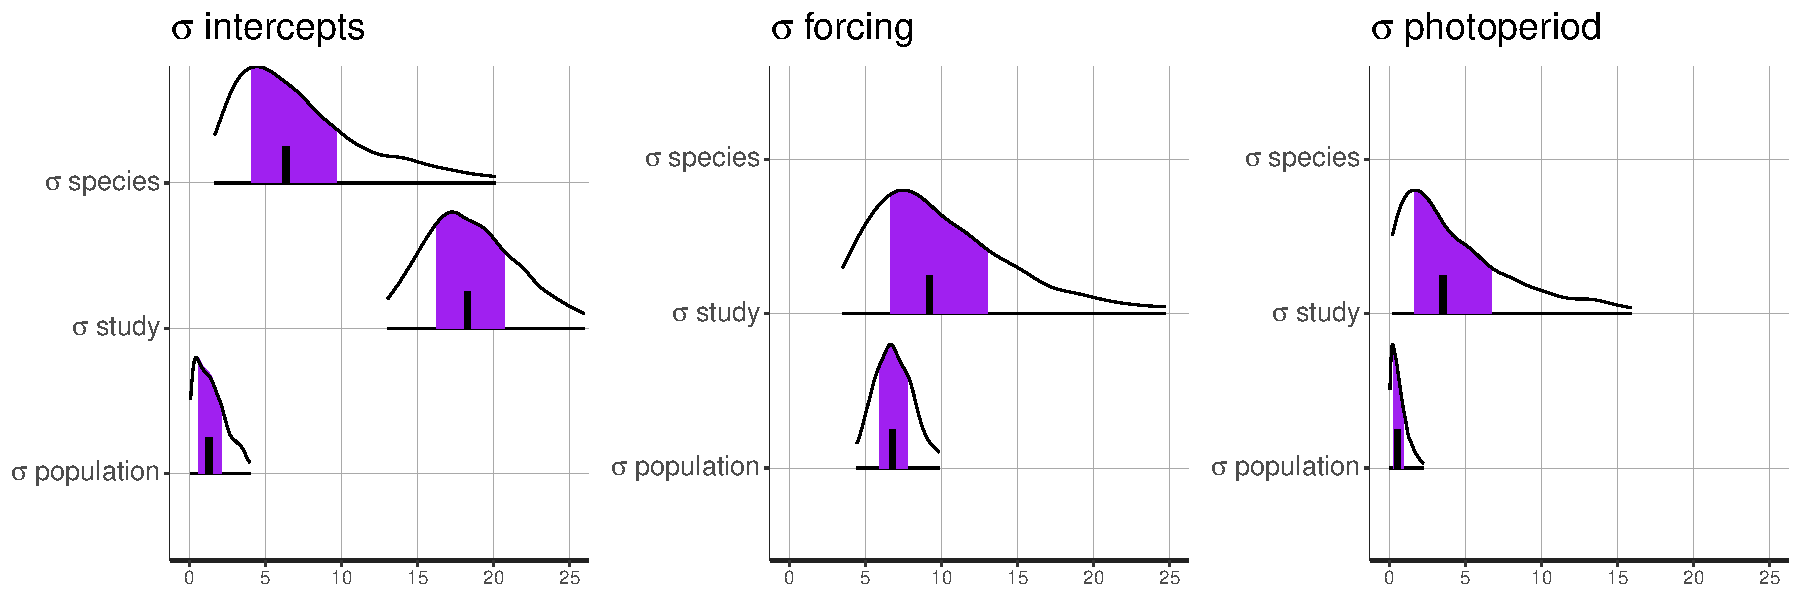
\includegraphics[width=\textwidth]{..//..//analyses/ranges/figures/variancepartitioning.pdf} 
    \caption{ \textbf{Local adaptation model estimates of variation partitioning in the intercept and forcing and photoperiod predictors using the OSPREE dataset}. For both the forcing and photoperiod predictors, within species (intraspecific) variation is much smaller than across species (interspecific) variation. Here we see that interspecific variation exceeds intraspecific variation at the intercept-level as well but variation at the study level is largest, suggesting experimental design is driving the highest level of uncertainty.}
    \label{fig:popy}
\end{figure}

\end{document}
